\vspace{1.5pc}
\section[Domain dan Data Penelitian]{Domain dan Data Penelitian}
\begin{spacing}{1.5}
	\subsection[Domain Penelitian]{Domain Penelitian}
	Penelitian ini mengkaji hubungan antara IOD, variabel oseanografi (arus, temperatur, salinitas, MLD, Chl-a, fluks air tawar, fluks panas bersih) dan meteorologi (laju presipitasi dan angin) di Samudera Hindia dengan koordinat ($0^\circ-24.6^\circ$ N) dan ($78.2^\circ-105^\circ$ E) (lihat Gambar \ref{fig:domain}).

	\subsection[Data Penelitian]{Data Penelitian}
%	\vspace{-1pc}
	Data yang digunakan dapat dilihat secara lengkap dalam Tabel \ref*{tab:data}.
	\begin{table}[H]
		\centering
		\caption{Rangkuman data penelitian}
		\label{tab:data}
		\begin{tabular}{|l|l|l|l|l|}
			\hline
			No & Data               & Periode   & Sumber      & Referensi \\ \hline
			1  & IOD                & 1994-2021 & AUSS        & AUSS      \\ \hline
			2  & Arus               & 1994-2021 & CMEMS/HYCOM & AUSS      \\ \hline
			3  & Temperatur laut    & 1994-2021 & CMEMS/HYCOM & AUSS      \\ \hline
			4  & Salinitas          & 1994-2021 & CMEMS/HYCOM & AUSS      \\ \hline
			5  & MLD                & 1994-2021 & CMEMS       & AUSS      \\ \hline
			6  & Chl-a              & 1994-2021 & CMEMS/MODIS & AUSS      \\ \hline
			7  & Fluks air tawar    & 1994-2017 & J-OFURO3    & AUSS      \\ \hline
			8  & Fluks panas bersih & 1994-2017 & J-OFURO3    & AUSS      \\ \hline
			9  & Laju presipitasi   & 1994-2021 & NCEP/NCAR   & AUSS      \\ \hline
			10 & Angin              & 1994-2021 & NCEP/NCAR   & AUSS      \\ \hline
		\end{tabular}
	\end{table}
	\subsection[Pengumpulan Data]{Pengumpulan Data}
	Data dalam Tabel \ref{tab:data} merupakan data yang tersedia secara gratis dan bersifat terbuka. Data ini dapat diunduh secara langsung pada website penyedia data ataupun menggunakan kode skrip. Kode skrip yang digunakan untuk mengunduh data dengan bahasa \textit{Shell script} (terminal Linux) dan Python disajikan dalam Lampiran 1.
	
	\begin{figure}[H]
		\centering
		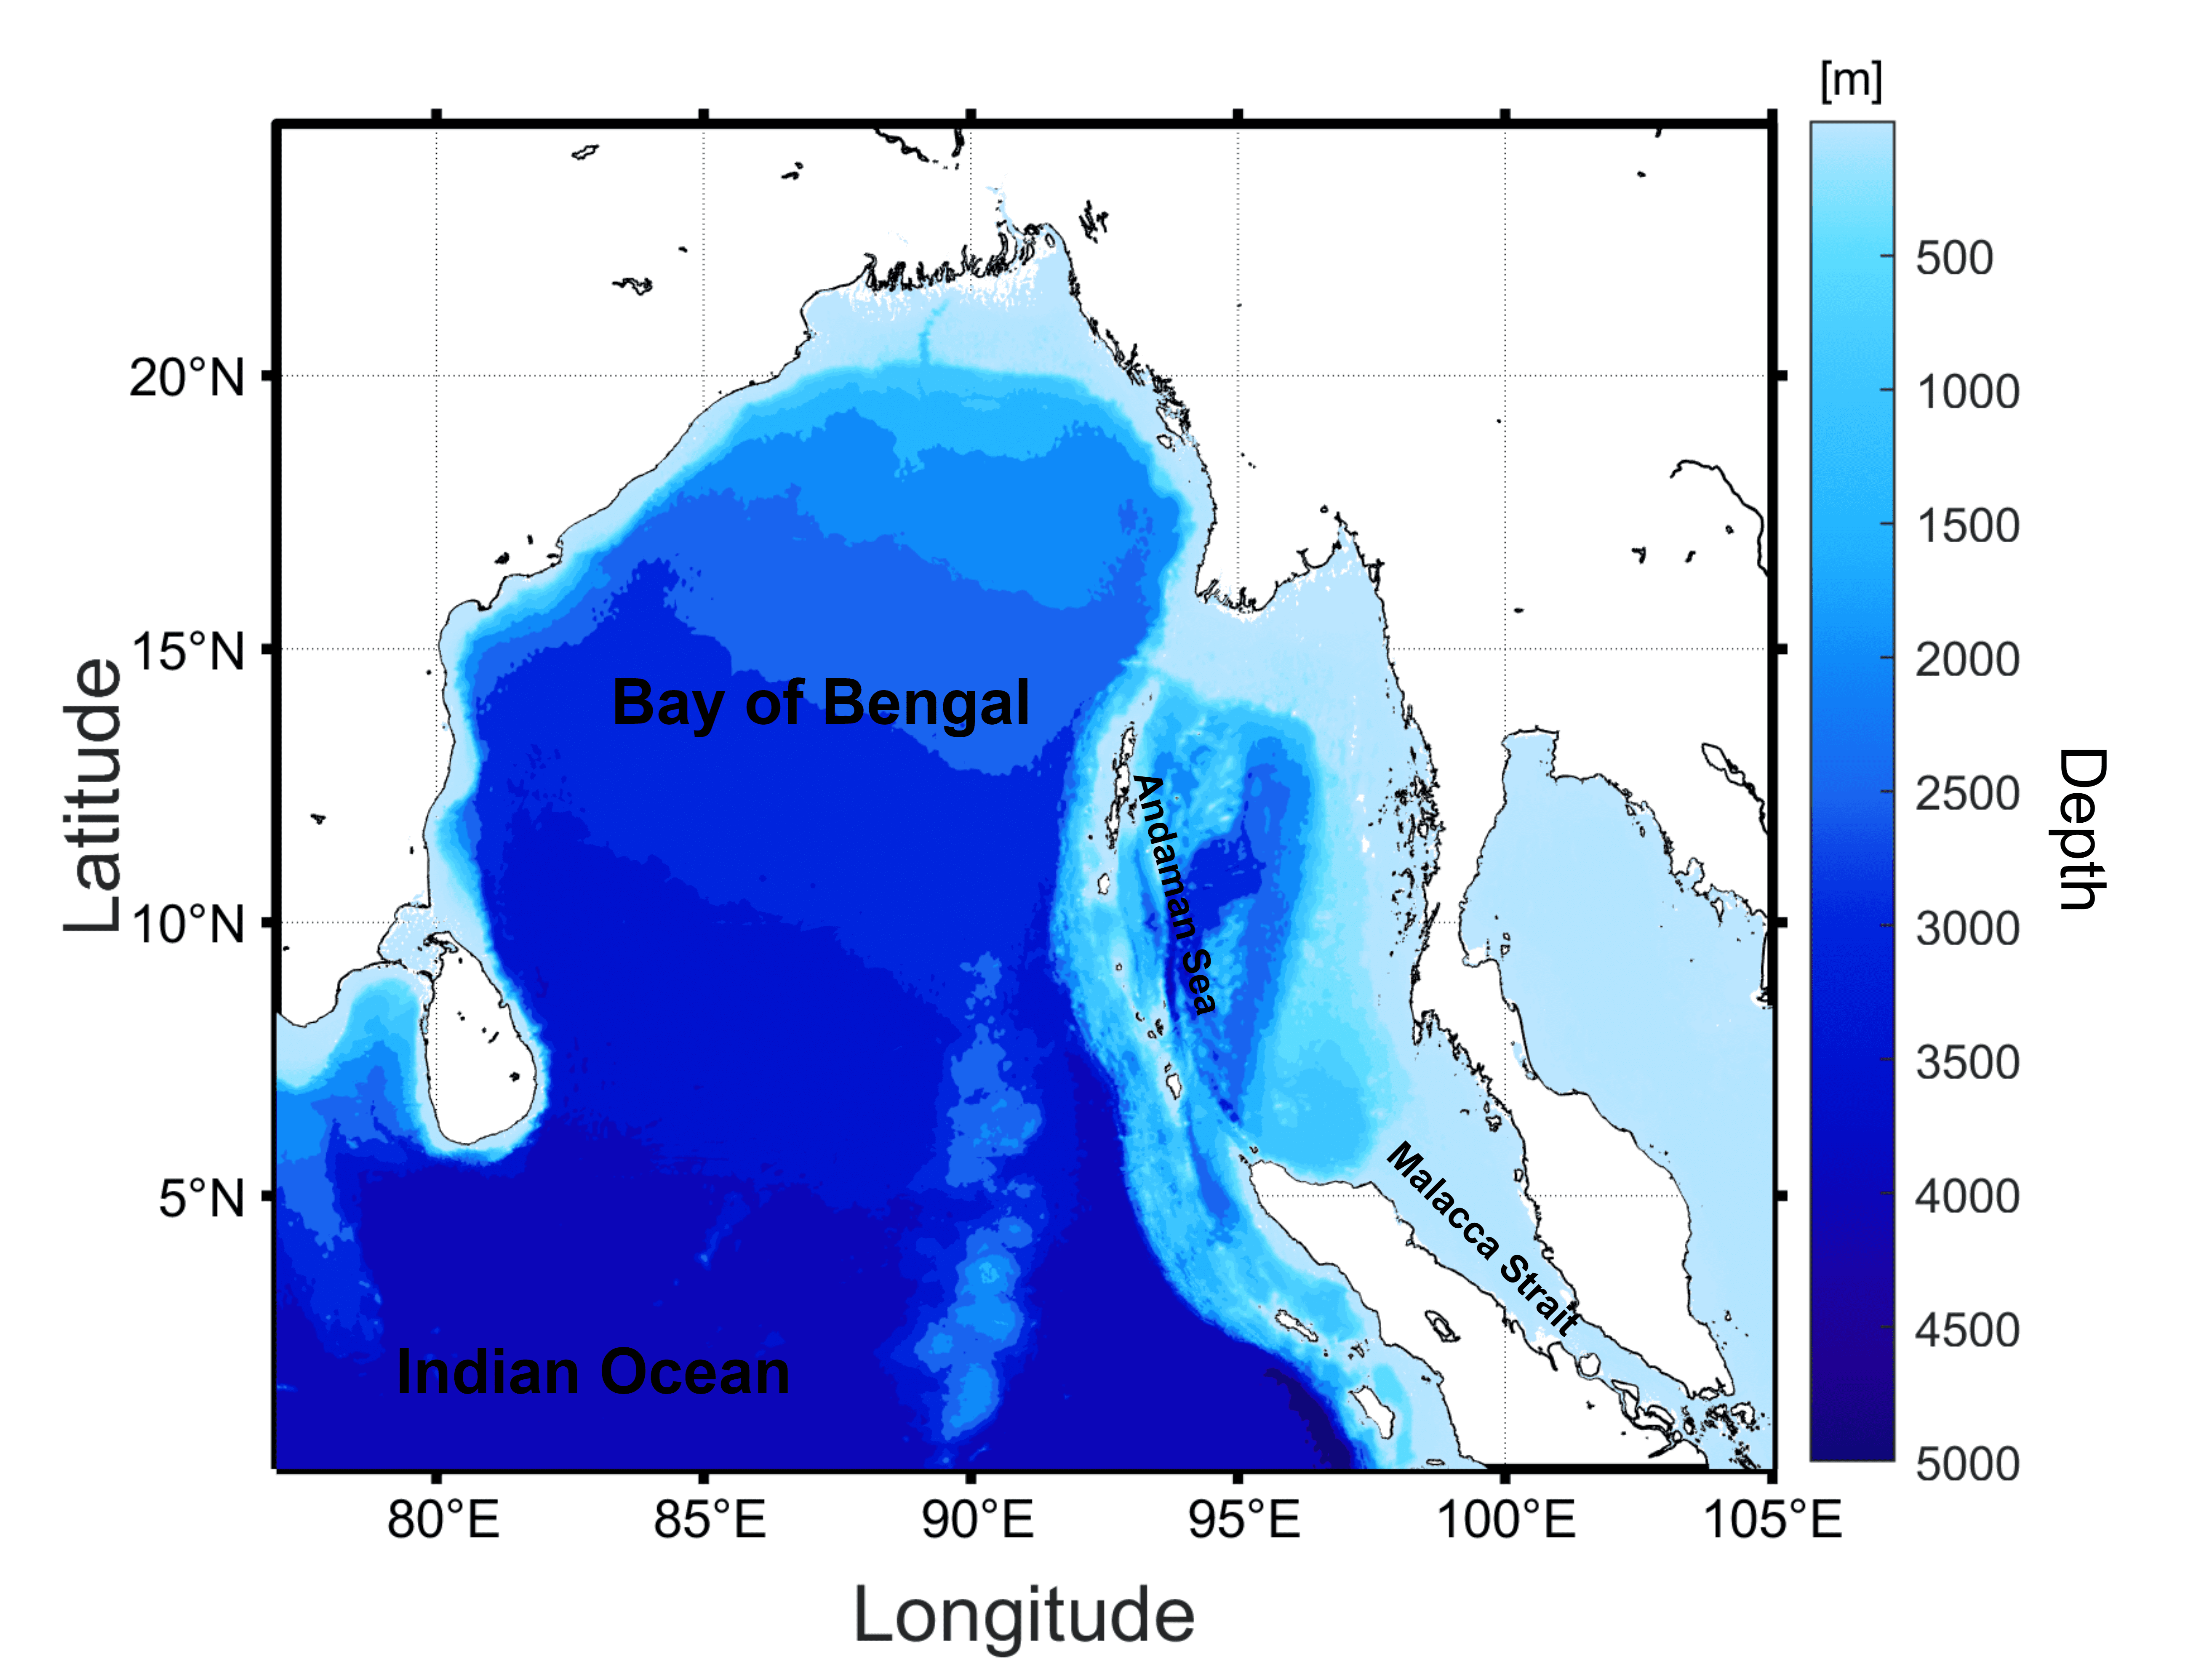
\includegraphics[width=12cm]{contents/Figures/Batimetri_edit_compress}
		\caption{Peta batimetri Samudera Hindia, diperoleh dari SRTM30+ \protect\cite{becker2009global}. Warna dalam peta menunjukkan kedalaman 0-5000 m sedangkan pulau digambarkan tanpa warna.}
		\label{fig:domain}
	\end{figure}
\end{spacing}
\vspace{-0.5pc}
\section[Analisis Data]{Analisis Data}
\begin{spacing}{1.5}
	\subsection[Model Musiman]{Model Musiman}
	Aplikasi deret waktu (\textit{time series}) banyak melibatkan data yang menunjukkan siklus musiman. Contoh yang paling umum digunakan adalah data cuaca. Dalam penelitian \shortciteauthor{Haridhi2016} \citeyear{Haridhi2016}, model nonlinear regresi digunakan untuk mengkarakterisasi hubungan antara SST (\textit{sea surface temperatur}) dan ND (\textit{net deployment}) - penyebaran jaring nelayan pukat cincin tradisional. Untuk menvalidasi temuan ini, mereka menggunakan persamaan siklus musiman \citeA{crawley2012r} dan mencari korelasi antara data SST dan data meteorologi. Dilain hal, \shortciteauthor{Ikhwan2022} \citeyear{Ikhwan2022} dalam penelitiannya mengkaji tentang kedalaman lapisan campuran (MLD) di laut Andaman menggunakan data salinitas (SSS) dari model 3-D CMEMS (\textit{Copernicus Marine Environment Monitoring Service}). Model iklim digunakan untuk mengidentifikasi dan memvalidasi jumlah musim MLD dalam setahun. 
	
	 Persamaan siklus musiman \cite{crawley2012r} dapat dituliskan sebagai
	\begin{equation}\label{eq:sm_}
		y = \alpha + \beta \sin(2\pi t)+\gamma \cos(2\pi t) + \epsilon,
	\end{equation}
	dengan $\alpha, \beta$, dan $\gamma$  adalah konstanta pergesaran vertikal, amplitudo dari gelombang sinus, dan amplitudo dari gelombang kosinus. Dalam persamaan ini, $t$ adalah waktu dan $\epsilon$ adalah elemen residual yang mewakili komponen \textit{white-noise} tidak beraturan dalam proses pengambilan data. 
	
	Gambar ini merupakan ilustrasi persamaan \ref{eq:sm_} untuk nilai $\alpha,\beta$ dan $\gamma$ yang berbeda. Nilai $\alpha$ yang berbeda mempengaruhi posisi kurva terhadap sumbu-y. Sedangkan nilai $\beta$ dan $\gamma$ yang berbeda mempengaruhi posisi kurva terhadap sumbu-x.
	\begin{figure}[H]
		\centering
		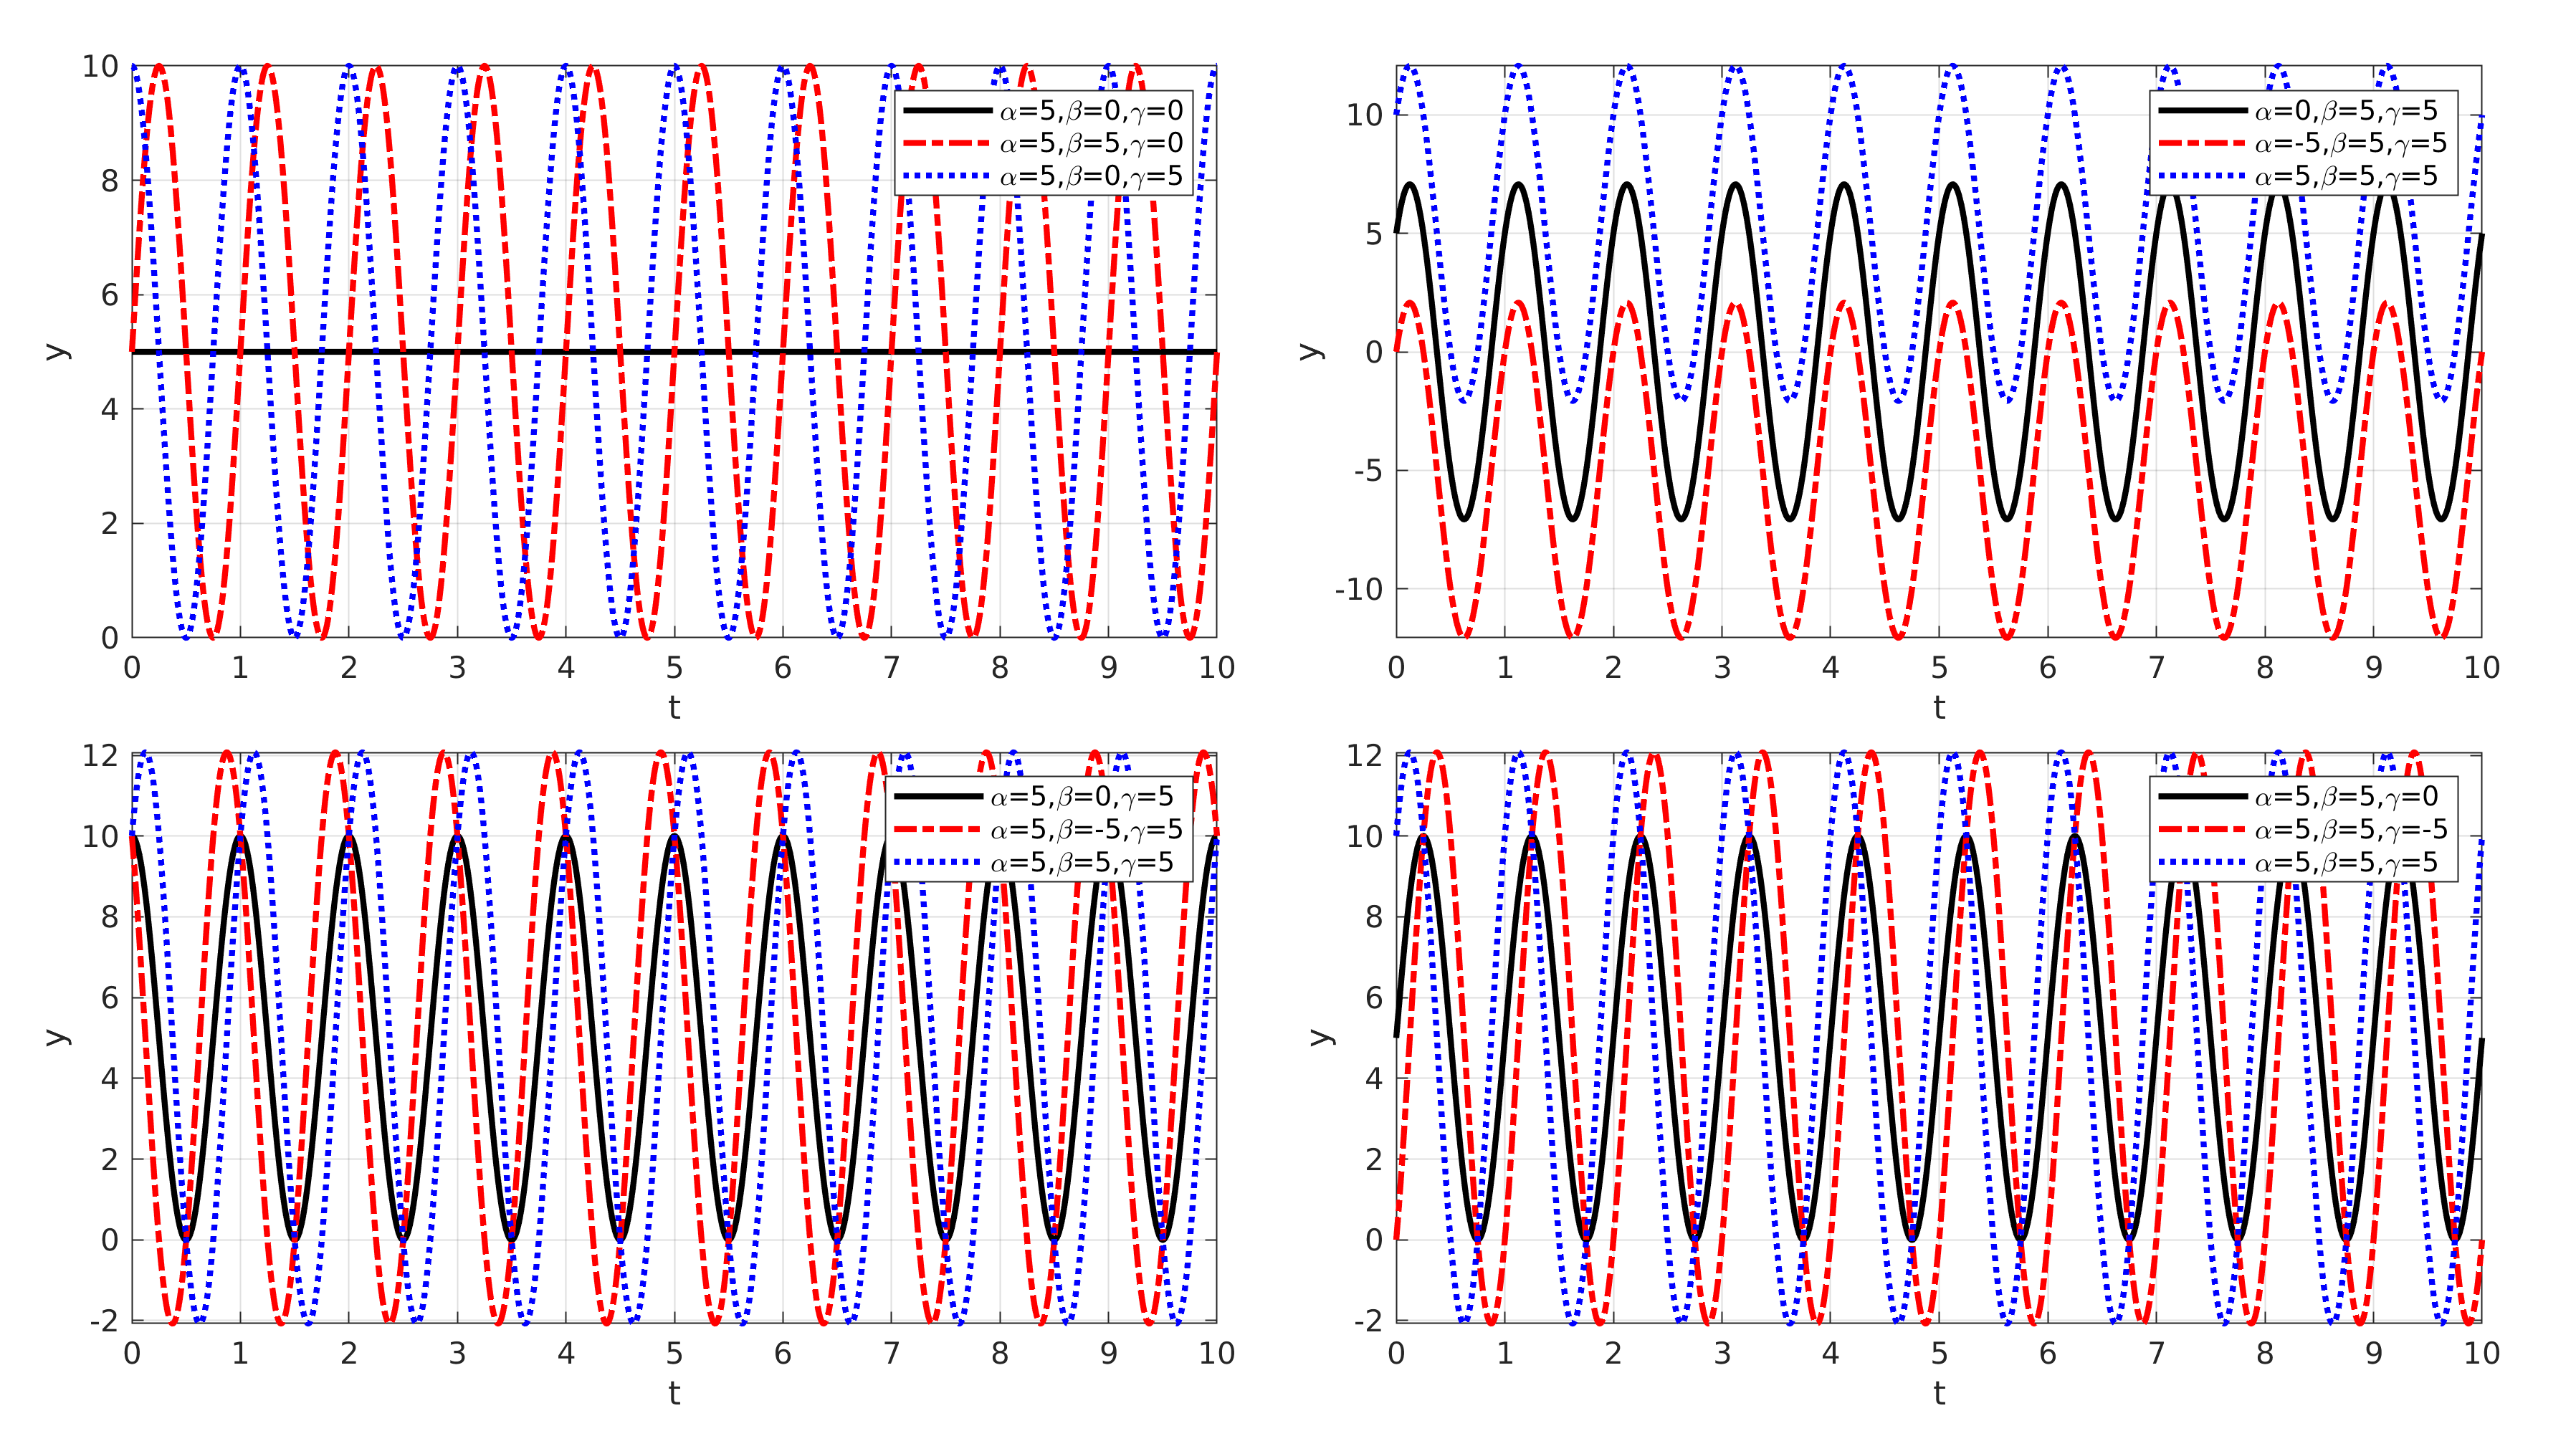
\includegraphics[width=15cm]{contents/Figures/sm_experiment}
		\caption{Ilustrasi persamaan model musiman.}
		\label{fig:sm}
	\end{figure}
	
%	Langkah-langkah yang digunakan untuk menggambarkan \textit{seasonal model} dapat dijelaskan sebagai berikut.
%	\begin{itemize}
%		\item \textbf{\textit{Start}}. \textit{Software} yang digunakan untuk menentukan nilai $\alpha, \beta$ dan $\gamma$ adalah \textit{software} \textit{R}.
%		\item \textbf{\textit{Initialization}}. Dalam proses inisialisasi ini, komponen musiman semua variabel dimodelkan untuk mendapatkan siklus tahunan.
%		\item \textbf{\textit{Input}}. Setelah proses inisialisasi \textit{input} variabel yang ingin diprediksi kemudian dimasukkan.
%		\item \textbf{\textit{Process}}. Selanjutnya dilakukan perhitungan dengan menggunakan fungsi model linear (\verb|lm()|) dalam \textit{R}.
%		\item \textbf{\textit{Output}}. Perintah Summary() digunakan untuk menampilkan hasil dalam proses sebelumnya. Dalam tahapan ini juga diperoleh penggambaran \textit{seasonal model}.
%	\end{itemize}

	\subsection[Analisis Korelasi]{Analisis Korelasi}
		Penelitian ini menganalisis hubungan antara IOD, variabel oseanografi (arus, temperatur, salinitas, MLD, Chl-a, fluks air tawar, fluks panas bersih) dan meteorologi (laju presipitasi dan angin). Persamaan korelasi dan koefisien korelasi yang digunakan dapat dituliskan sebagai \cite{hidayat2023relationship,Haditiar2020}
		\begin{equation}
			\begin{aligned}
				y &= a+rx\\
				r &= \frac{\sum (x_i - \bar{x})(y_i - \bar{y})}{\sqrt{\sum (x_i-\bar{x})^2\sum (y_i-\bar{y})^2}},
			\end{aligned}
		\end{equation}
		dengan $\alpha$ adalah konstanta titik potong sumbu-$y$, $r$ adalah kemiringan dari garis regresi (koefisien regresi), $x_i, y_i$ adalah variable yang digunakan untuk menghitung koefisien korelasi dengan $i$ adalah indeks data. Sedangkan $\bar{x}$ dan $\bar{y}$ adalah rata-rata. 
		
\end{spacing}
\vspace{-0.5pc}
\section[Prosedur Penelitian]{Prosedur Penelitian}
\begin{spacing}{1.5}
	Prosedur penelitian mengikuti diagram alir pada Gambar \ref{fig:flowchart} dan dapat dijelaskan sebagai berikut. 
	\begin{itemize}
		\item \textbf{\textit{Start}}. \textit{Software} yang digunakan dalam penelitian ini adalah Matlab dan \textit{R}.
		\item \textbf{\textit{Input}}. Data-data terkait penelitian yang akan digunakan sebagai \textit{input} diunduh terlebih dahulu.
		\item \textbf{\textit{Process}}. Setelah data tersedia, kemudian data diolah dengan cara melakukan pemetaan dan penggambaran data.
		\item \textbf{\textit{Output}}. Hasilnya adalah peta IOD, oseanografi, dan meteorologi secara jangka panjang. 
		\item \textbf{\textit{Process}}. Tahapan selanjutnya adalah analisis data. Dalam tahap ini dilakukan analisis model musiman (\textit{seasonal model}) untuk mengidentifikasi pola musiman dan memprediksi variabel berdasarkan keteraturannya. Dilakukan juga analisis statistik, dalam hal ini analisis korelasi untuk melihat hubungan IOD, variabel oseanografi dan meteorologi.
		\item \textbf{\textit{Output}}. Terakhir, diperoleh kesimpulan berdasarkan analisis yang telah dilakukan.
		\item \textbf{\textit{End}}. Penelitian selesai.
	\end{itemize}
	\begin{figure}[H]
		\centering
		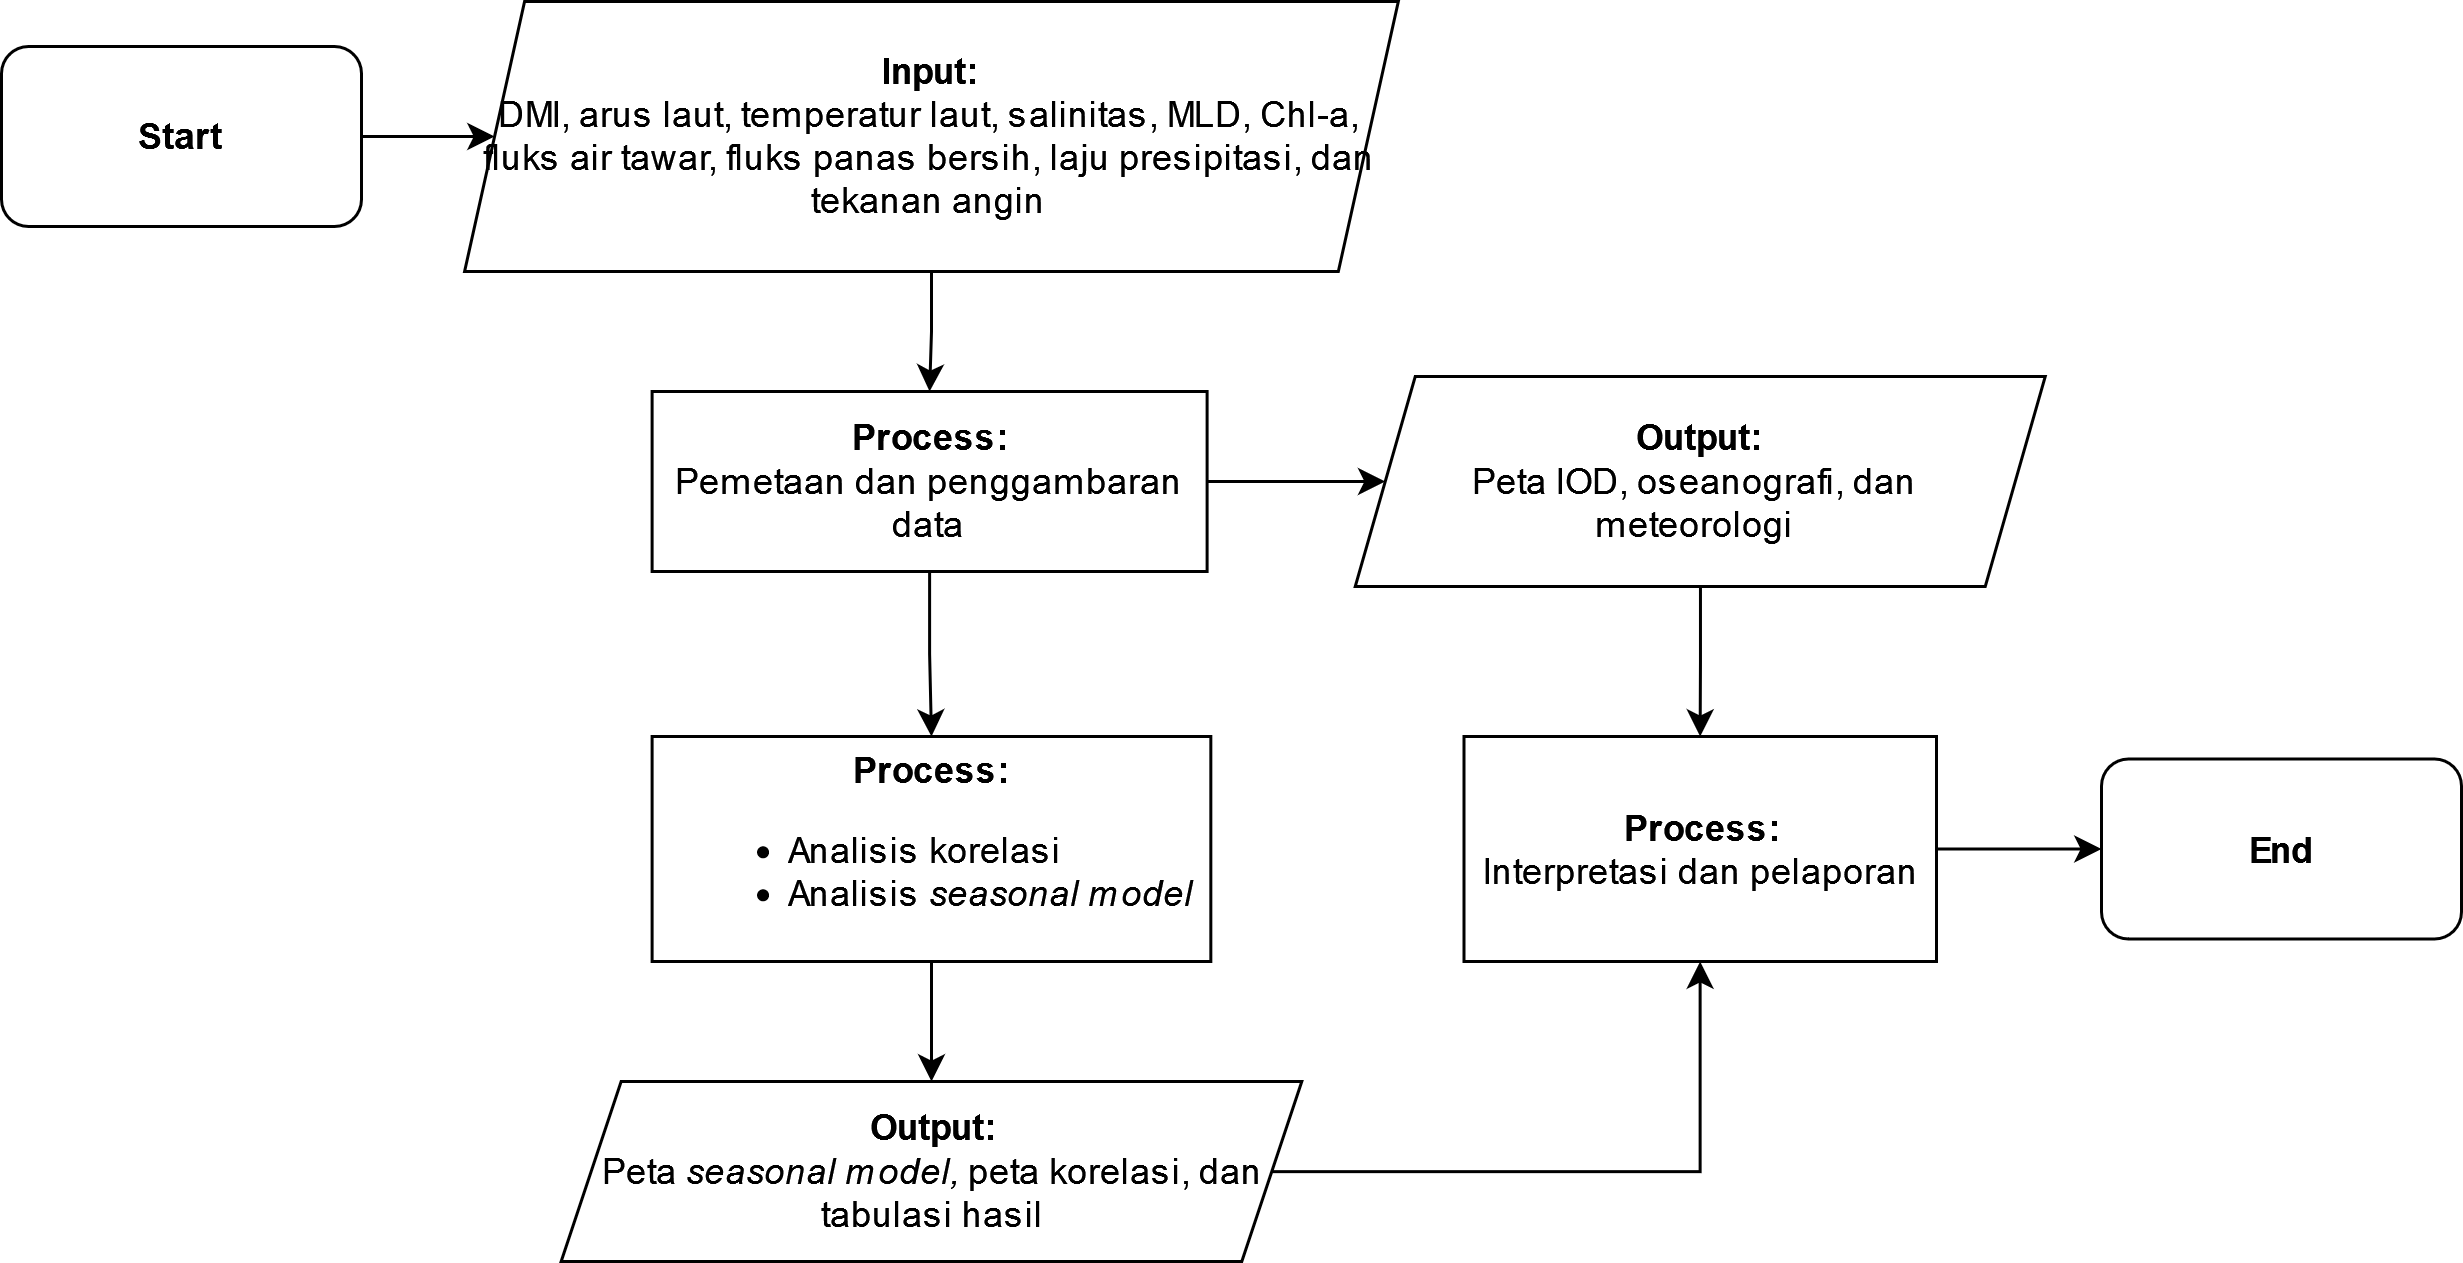
\includegraphics[width=10cm]{contents/Figures/Flowchart_Diagram.png}
		\caption{Diagram alir penelitian}
		\label{fig:flowchart}
	\end{figure}
\end{spacing}
